\documentclass[10pt]{article}
\usepackage[utf8]{inputenc}
\usepackage{url}
\usepackage{hyperref}
\usepackage{amsmath}
\usepackage{amsfonts}
\usepackage{amssymb}
\usepackage{graphicx}
\usepackage{float}
\usepackage{multicol}
\usepackage{xcolor}
\usepackage{natbib}
\usepackage{tikz}
\usetikzlibrary{positioning,arrows.meta}
\usepackage[font=small]{caption}
\addtolength{\abovecaptionskip}{-3mm}
\addtolength{\textfloatsep}{-5mm}
\setlength\columnsep{20pt}

\usepackage[a4paper,left=1.50cm, right=1.50cm, top=1.50cm, bottom=1.50cm]{geometry}

\newcommand{\cl}[1]{\texttt{#1}}

\author{Jeff Barner}

\title{Evidential Fusion for Calibrated Edge Traversability on a Wheeled Delivery Robot}

\begin{document}

	\begin{center}
		{\Large \textbf{Evidential Fusion for Calibrated Edge Traversability on a Wheeled Delivery Robot}}\\
		\vspace{1em}
		{\large Jeff Barner}\\
		\vspace{1em}
		\textit{Department of Electrical and Computer Engineering, Rutgers University}
	\end{center}


	\begin{center}
		\rule{150mm}{0.2mm}
	\end{center}

	\begin{abstract}

	A sidewalk delivery robot follows a route from a map, but maps go stale: a path marked as a walkway
	may contain stairs or a curb that a wheeled robot cannot cross. Camera and LiDAR can catch the error,
	but each fails in its own way. This project combines camera, LiDAR, and map into one \emph{confidence}
	that a path segment is safe, which also reports its uncertainty and when the sources disagree. The robot
	crosses only on trustworthy confidence, looks closer when unsure, and reroutes around hazards. Evaluation
	replays real campus robot logs with injected stale maps and adversarial camera evidence.

	\textbf{Collaborators}: Dr. Jorge Ortiz, Rutgers University
	\end{abstract}

	\begin{center}
		\rule{150mm}{0.2mm}
	\end{center}

	\vspace{1mm}

\begin{multicols*}{2}

\section{Problem and Decision Boundary}

A wheeled delivery robot follows a campus sidewalk graph whose edge labels come from a map prior
(OpenStreetMap~\cite{osm}). Labels can be stale: an edge tagged \cl{footway} may contain stairs or a curb.

\textbf{Decision:} for each edge $e$ on the route, may the robot commit to traversing it?
\begin{itemize}\setlength\itemsep{0pt}\setlength\parskip{0pt}
	\item \textbf{Act:} traverse $e$.
	\item \textbf{Defer:} an obligation is unresolved and closer observations remain; re-observe.
	\item \textbf{Repair:} an obligation fails; remove $e$, replan, record a map patch.
	\item \textbf{Handoff:} no admissible route remains; escalate to an operator.
\end{itemize}
Admitting a curb or stairs is catastrophic, while a false rejection costs a detour, so the gate is
fail-closed.

\textbf{Research question:} does extending evidential multi-view fusion (TMC~\cite{han2023}) to discount
the map's reliability by label age and accumulate evidence over the approach give better-calibrated edge confidence
than softmax fusion and standard TMC, and can a gate on it match a ``reject if any source objects'' veto
on false admission with fewer unnecessary rejections? Perception is out of scope: views are frozen,
cached features.

\begin{center}
	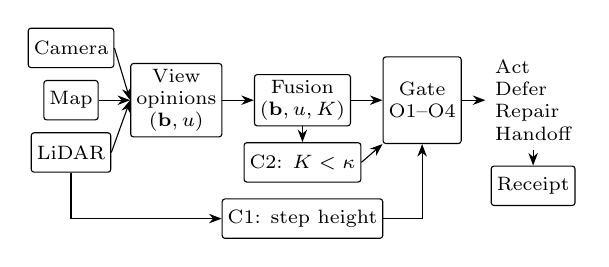
\begin{tikzpicture}[font=\scriptsize, >={Stealth[length=1.6mm]},
		box/.style={draw, rounded corners=1pt, align=center, inner sep=2pt, minimum height=5mm},
		node distance=3mm and 4mm]
		\node[box] (cam) {Camera};
		\node[box, below=1.5mm of cam] (map) {Map};
		\node[box, below=1.5mm of map] (lid) {LiDAR};
		\node[box, right=of map] (op) {View\\opinions\\$(\mathbf{b},u)$};
		\node[box, right=of op] (fus) {Fusion\\$(\mathbf{b},u,K)$};
		\node[box, right=of fus, minimum height=11mm] (gate) {Gate\\O1--O4};
		\node[box, below=2mm of fus] (c2) {C2: $K<\kappa$};
		\node[box, below=2mm of c2] (c1) {C1: step height};
		\node[align=left, right=3mm of gate] (out) {Act\\Defer\\Repair\\Handoff};
		\node[box, below=2mm of out] (rec) {Receipt};
		\foreach \v in {cam,lid,map} \draw[->] (\v.east) -- (op.west);
		\draw[->] (op) -- (fus);
		\draw[->] (fus) -- (gate);
		\draw[->] (fus) -- (c2);
		\draw[->] (c2.east) -- (gate.south west);
		\draw[->] (lid.south) |- (c1.west);
		\draw[->] (c1.east) -| (gate.south);
		\draw[->] (gate) -- (out);
		\draw[->] (out) -- (rec);
	\end{tikzpicture}
	\captionof{figure}{Per-view opinions are fused, checked by C1 and C2, and gated; every decision is logged to the receipt.}
	\label{fig:pipeline}
\end{center}

\section{Modalities, Data, Typed Claims, Risks, and Obligations}

\textbf{Data:} \emph{GND}~\cite{liang2025} (CC0), which includes a labeled traversability map.
Training uses UMD map~3 (McKeldin Mall), split by location; Georgetown is held out. Bags hold LiDAR,
RGB, odometry, and SLAM poses, and are cached once, so no network is needed afterward. Edges are
labeled \emph{traversable} or \emph{hazard} (GND's stairs-or-curb class); a curb and stairs both mean a reroute.

\textbf{Typed claims:} each view turns its feature into an opinion $(\mathbf{b}, u)$ over the two
classes, and the edge is classified from the \emph{fused} opinion (Table~\ref{tbl:claims}). The map
is never certain: its opinion is discounted by label age, $\mathbf{b}' = r\mathbf{b}$, $u' = 1 - r(1-u)$,
with $r = r_{\max} e^{-\text{age}/\tau_a}$ and $r_{\max} < 1$, so an old label adds uncertainty, not hazard belief. Every claim records edge, value, uncertainty, source, tier, and
provenance (sensor, timestamp, range, artifact hash, version).

\begin{table*}
	\centering
	\small
	\begin{tabular}{lll}
		\hline
		\textbf{Source (frozen feature)} & \textbf{Example claim} & \textbf{Role} \\
		\hline
		Camera (DINOv2~\cite{oquab2024dinov} embedding) & \cl{terrain(e): b=(.15,.70), u=.15} & Semantic evidence (A1) \\
		LiDAR (step-height histogram) & \cl{terrain(e): b=(.05,.81), u=.14} & Geometric evidence \\
		Map prior (OSM tag, 5-year-old label) & \cl{terrain(e): b=(.58,0), u=.42} & Age-discounted prior \\
		Fusion (TMC / proposed) & \cl{b=(.12,.85), u=.02, K=.47} & Fused opinion (A2) \\
		C1 step height (raw points) & \cl{max\_step(e)=0.14\,m, n=812} & Executable checker \\
		\hline
	\end{tabular}
	\caption{Example typed claims on a stale edge mapped as \cl{footway} that has stairs; $\mathbf{b}$ = (traversable, hazard). $K$ is the largest conflict between view opinions, used by checker C2.}
	\label{tbl:claims}
\end{table*}

\textbf{Risk tiers} set how much evidence Act needs, from OSM context known before arrival:
\textbf{T0} interior walkway; \textbf{T1} meets a roadway or crossing (likely curb); \textbf{T2} within
$d$\,m of mapped steps or kerbs. An edge escalates to T2 if its fused hazard belief ever reaches $\beta$.

\textbf{Obligations:} any \textsc{fail} $\Rightarrow$ Repair; any \textsc{unresolved} $\Rightarrow$ Defer,
or Repair if no closer evidence remains.
\begin{itemize}\setlength\itemsep{0pt}\setlength\parskip{0pt}
	\item \textbf{O1} (all): view conflict $K < \kappa$ (C2).
	\item \textbf{O2} (T1+): max step $< 0.05$\,m with enough points (C1); for T2, on $\ge 2$ frames at different ranges.
	\item \textbf{O3} (all): fused $b_{\text{trav}} \ge \tau_{\text{tier}}$ and $u \le \tau_u$.
	\item \textbf{O4} (all): every claim resolves to a hashed artifact.
\end{itemize}

\textbf{Risks:} few hazard sites (counted first); OSM edit time is not survey time; Dempster's rule hides stale-map conflict; C1 and the
LiDAR view share a sensor.

\section{CPU Baseline: Estimated Runtime and Memory}

Estimates on 4 cores and 16\,GB for $\sim$3.7k frames at 2\,Hz; measured values go to \cl{compute.json}.

\begin{center}
	\footnotesize
	\begin{tabular}{@{}lrr@{}}
		\hline
		\textbf{Stage} & \textbf{Time} & \textbf{RAM} \\
		\hline
		Bags (72\,GB) $\to$ 2\,Hz cache, once & 65\,min & $<$2\,GB \\
		Graph, association, labels & $<$5\,min & $<$2\,GB \\
		Frozen features, C1 & 10\,min & 3\,GB \\
		Fusion ladder (9 methods $\times$ 5 seeds) & $<$10\,min & $<$2\,GB \\
		Gate and receipts & 20\,min & $<$3\,GB \\
		\hline
		Baseline / evaluator & 1.8\,h / 30\,min & $<$6\,GB \\
		\hline
	\end{tabular}
\end{center}

Both fit the 4\,h / 2\,h budgets. \textbf{Minimum fallback:} LiDAR and map views with fixed
Dempster--Shafer masses~\cite{valente2018}, plus C1 and C2.

\section{Checkers, Action Gate, Invariant, and Failure Injection}

\textbf{C1, geometric step height:} fits a ground plane to raw LiDAR points on the edge
(RANSAC~\cite{ransac1981}) and reports the largest step. No learning.

\textbf{C2, fusion conflict:} reports the largest Dempster conflict between pairs of view opinions.
It reads only opinions, never geometry, and flags the disagreement a stale map creates.

\textbf{Gate:} a deterministic function of claims and tier. Missing evidence is \textsc{unresolved},
never \textsc{pass}. Deferral consumes the next, closer cached frame.

\textbf{Invariant I1:} no edge is admitted unless every obligation for its tier passes. It is checked on
every receipt and by property-based tests.

\textbf{Receipt:} config and data hashes, seed, faults, and per-edge claims, obligations, and decision.

\textbf{Failure injection} (expected detection in parentheses):
\begin{itemize}\setlength\itemsep{0pt}\setlength\parskip{0pt}
	\item \emph{Stale map:} stair and curb edges flipped to \cl{footway} with assigned label ages (C2 conflict).
	\item \emph{Adversarial:} stale map plus flat-sidewalk crops swapped in for stairs (only the LiDAR view and C1 remain).
\end{itemize}

\textbf{Unwarranted claims:} none about real-world safety, other campuses, hazards beyond steps and
stairs, or physical causation.

\section{Metrics, Baselines, Ownership, Timeline, and Fallback}

\textbf{Task performance:} ECE, NLL, hazard F1, AUROC for stale-edge detection, and risk--coverage.

\textbf{Fusion baselines:} map only; single view; early, late, and attention fusion (A2); fixed
Dempster--Shafer masses~\cite{valente2018}; TMC~\cite{han2023} and QMF~\cite{zhang2023}; proposed.

\textbf{Policy behavior:} false admission (Wilson CI), unnecessary rejection and deferral, checker
coverage, failure detection, repair success (goal reached using only truly traversable edges; detour
overhead vs.\ an oracle map), runtime, and peak memory. Policies: map-only route, conservative veto,
gate on TMC, gate on proposed fusion.

\textbf{A1/A2/A3:} cached embeddings (A1); evidential opinions with conformal
thresholds~\cite{Angelopoulos2021} (A2); per-decision attribution by ablating each view (A3).
\textbf{Ownership:} solo.

\textbf{Timeline:} \emph{Nov 7--20:} cache, labels, features, C1, baselines.
\emph{Nov 21--30:} C2, gate, receipts, one injection. \textbf{Dec 1 progress gate.}
\emph{Dec 2--10:} proposed fusion, all injections, A3, poster. \emph{Dec 12--15:} report.

\textbf{Fallbacks:} proposed loses to TMC
$\Rightarrow$ gate on TMC; UMD alignment or association fails $\Rightarrow$ Georgetown becomes primary.

\textbf{Repository:} \url{https://github.com/nalddox/ml4ss-terrain-gate}.
\textbf{Data access:} GND UMD map~3 north (chunks 01--15), Georgetown, and both traversability
maps are downloaded locally. \textbf{Optional scale-up:} none requested; everything runs on CPU.

\end{multicols*}

\clearpage

\bibliography{../ref/ref}
\bibliographystyle{plainnat}

\end{document}
